\documentclass[12pt,a4]{article}
\pagestyle{plain}                           

% Use Report Template
\usepackage{temp/report_template}

% For appendix
\usepackage[toc,page]{appendix}

% For Better Tables
\usepackage{tabularx}

% For Fortran Code
\usepackage{listings}
\lstset{language=[90]Fortran,
  basicstyle=\ttfamily,
  keywordstyle=\bfseries,
  commentstyle=\itshape,
  morecomment=[l]{!\ },% Comment with only space after !
  showstringspaces=false,
  frame=topline
}

% For Subfiles
\usepackage{subfiles}

% Graphics Path
\graphicspath{{img/}{../img/}}

% Indent
\setlength\parindent{1 in}

\begin{document}
\title{Na\"ive Tsunami Generation via Shallow Water Theory\\
\large  MATH484 Final Project Report}
\author{Lonny Cox-Lauf, Jonah Kopp, Clay Kramp, John Luke Lusty}
\date{May 8\textsuperscript{th} 2018}

\begin{titlepage}
	\maketitle
    \begin{figure}[h]
        \centering
        \fbox{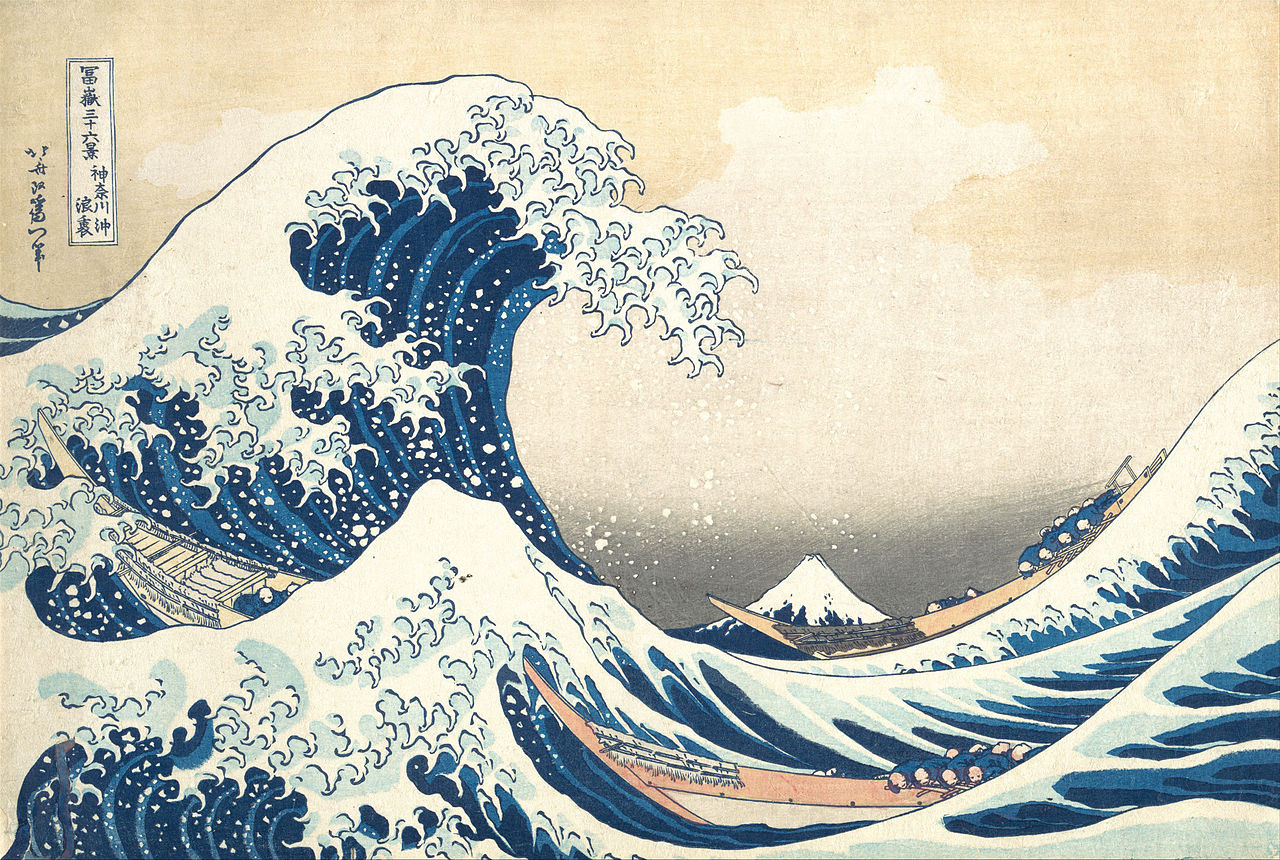
\includegraphics[width=\textwidth]{great_wave}}
        \caption*{\textit{"The Great Wave off Kanagawa"}, Katsushika Hokusai est. 1829}
    \end{figure}
\end{titlepage}
	
\tableofcontents
\pagebreak

% INTRODUCTION
\section{Introduction}
\subfile{sec/intro}

% SHALLOW-WATER THEORY
\section{Shallow-Water Theory}
\subfile{sec/shallow}

% CONSERVATIVE FORM
\section{The Conservative Form of a Hyperbolic Equation}
\subfile{sec/conserve}

% NUMERICAL METHODOLOGY
\section{Numerical Methodolgy}
\subfile{sec/numerics}

% APPLICATION
\section{Application: Fukushima Daiichi Nuclear Disaster}
\subfile{sec/app}

% BEZIER
\section{Interpolating Sea Floor: Fukushima Daiichi Nuclear Disaster}
\subfile{sec/bezier}

% RESULTS
\section{Results }
\subfile{sec/results}

%CONCLUSION
\section{Conclusion}
\noindent The shallow-water wave equation provides a strong starting point for analyzing the propagation and growth of waves over a known sea floor (or any surface supporting a body of water). However, in order to achieve this desired result we had to make several assumptions. The perturbation that we use to represent the initial state of the tsunami is not representative of nature. In nature, we would expect a pressure wave emanating radially from the epicenter to propagate evenly in all directions. This would lead to a much shorter initial wave (which may still be Gaussian, just with a larger sigma parameter), and the water beneath the surface wave would also have behavior significant to the generation of the tsunami. Essentially, a more accurate model would account for a pressure wave beginning at the epicenter and expanding evenly in all directions, showing more behavior than just at the surface.\\

\noindent Despite the limitations of the model as-is, we achieved our goal of numerically solving the shallow-water wave equation in one dimension given the shape of the sea floor below. We were also able to apply a new sort of boundary condition, a radiation condition, which allowed the wave to leave the system without reflecting back in. This worked much better than our initial attempt of using Dirichlet boundary conditions, setting the height of the wave to $0$. This first attempt introduced significant numerical instability.\\

\noindent Going forward, we would like to see our method implemented in 2D. We finished creating the smooth 2D sea floor and finding the $x$ and $y$ derivatives, but did not implement the Lax-Wendroff numerical scheme in 2D. Additionally, we would like to take steps to make this simulation closer to what would be observed in nature--perhaps starting the simulation before the earthquake occurs, having a model that can handle a rapid shift of the sea floor. An integral formulation of the equation may be able to handle such discontinuities. \\

\noindent Our na\"ive approach to the generation of tsunamis may not have been exactly representative of nature, but the growing height of the wave as it approached the shore is an accurate representation of how the sea floor affects approaching waves. Adjusting the parameters and initial perturbation may facilitate more accurate simulations, allowing for rough approximations to tsunamis all over the world, provided the sea floor elevation data is readily available.

\begin{thebibliography}{1}
\bibitem{zirker}
Jack B Zirker.
\textit{The Science of Ocean Waves: Ripples, Tsunamis, and Stormy Seas}.
John Hopkins University Press, 22 October 2013. 
Accessed via Arthur Lakes Library at the Colorado School of Mines, March 31, 2018.
    
\bibitem{marghany}
Maged Marghany.
\textit{Simulation of Tsunami Impact on Sea Surface Salinity along Banda Aceh Coastal Waters, Indonesia}.
Advanced Geoscience Remote Sensing, Ch 3. Intech, 2014. Accessed via In Tech Open, March 31, 2018.
    
\bibitem{satake1}
Yuichiro Tanioka, Kenji Satake.
\textit{Tsunami generation by horizontal displacement of ocean bottom}.
Geophysical Research Letters, Vol 3, No 8, 15 April 1996. American Geophysical Union Publications. Accessed via Wiley Online Library, March 31, 2018.

\bibitem{salmon}
Rick Salmon.
\textit{Introduction to Ocean Waves}.
Scripps Institution of Oceanography, University of California, San Diego, 7 December 2015. Accessed via Rick Salmon's website via http://pordlabs.ucsd.edu/rsalmon/, March 31, 2018.

\bibitem{rezzolla}
Luciano Rezzolla.
\textit{Lecture Notes on Numerical Methods for the Solution of Hyperbolic Partial Differential Equations}.
SISSA, International School of Advanced Studies, Trieste, Italy, 2 August 2015. Accessed via Luciano Rezzolla's website via http://www.sissa.it/~rezzolla, March 31, 2018.

\bibitem{nuclearAssociation}
World Nuclear Association.
\textit{Fukushima Accident}.
October, 2017. Accessed via http://www.world-nuclear.org/information-library/safety-and-security/safety-of-plants/fukushima-accident.aspx, May 3, 2018.

\end{thebibliography}
	
\end{document}
